\chapter{Suma de red}
\label{chap:latticesum}

Lo que sigue es una adaptación del capítulo F del Ashcroft.

Tratamos de demostrar que
\begin{equation*}
\sum_\mathbf{R} e^{-i\mathbf{k}\mathbf{R}}=N {\delta(\mathbf{k},\mathbf{G})}
\end{equation*}
donde $\mathbf{R}$ corre por los $N$ sitios de la red de Bravais:
\begin{equation*}
  \mathbf{R} = \sum_{i=1}^{3} n_i \mathbf{a}_i \ ; \ \ n_i \in [0,N)
\end{equation*}
La suma ha de ser igual si desplazamos todos los $\mathbf{R}$ la misma
cantidad, ya que cumple las condiciones de contorno de Born-von
Karman. En palabras de la todopoderosa Wikipedia:
\begin{quotation}
  \emph{The Born–von Karman boundary condition are periodic boundary
    conditions which impose the restriction that a wave function must be
    periodic on a certain Bravais lattice.}
\end{quotation}

Por tanto, suponiendo $\mathbf{R_0}$ un vector de la red cualquiera,
\begin{equation*}
 \sum_\mathbf{R} e^{-i\mathbf{k}\mathbf{R}} = \sum_\mathbf{R}
 e^{-i\mathbf{k}(\mathbf{R} - \mathbf{R_0})} =  e^{i \mathbf{k} \mathbf{R_0}}\sum_\mathbf{R} e^{-i\mathbf{k}\mathbf{R}}
\end{equation*}
Esta última ecuación se cumple en dos casos:
\begin{itemize}
\item Si la suma $ \sum_\mathbf{R} e^{-i\mathbf{k}\mathbf{R}}$ es nula.
\item Si $e^{i \mathbf{k} \mathbf{R_0}}$ es la unidad.
\end{itemize}

Si $e^{i \mathbf{k} \mathbf{R_0}}$, $\mathbf{k}$ es un vector de la
red recíproca. Por tanto, la suma valdrá $N$ si se cumple que
$\mathbf{k} \in \{ \mathbf{G} \}$ o se anulará en caso
contrario. $\blacksquare$

\chapter{Dependencia térmica de $\boldsymbol{\kappa}$}
\label{app:thermaldep}

\section{Calor específico}
En los aislantes la única contribución a $c_v$ es la red. Los modelos
de Einstein y Debye (ver más en \ref{sec:cvlattice}) predicen que la
contribución al calor específico de los fonones es constante a alta temperatura (ley de
Dulong-Petit) y proporcional a $T^3$ a baja temperatura (predicho por
el modelo de Debye).
\begin{equation*}
  \boxed{
  \begin{cases}
    c_v^\text{ph.} (T \ll \theta_D) \propto& T^3 \\
    c_v^\text{ph.} (T \gg \theta_D) =& \text{cte.}
  \end{cases} }
\end{equation*}
En los metales existe una contribución extra debida a los electrones,
de menor valor (fig. \ref{fig:electronvsphononcv}).
Utilizando que para un gas de Fermi la densidad de estados viene dada por
$D(\varepsilon_F) = \frac{3N}{2\varepsilon_F}$, con la expansión de
Sommerfield hallamos
\begin{equation*}
  U(T) = U(0) + \frac{\pi^2}{6} (\kb  T)^2 D(\varepsilon_FT) \
  \rightarrow \ c_v^e = \frac{\pi^2 \kb ^2 N}{2\varepsilon_F}T = \gamma T 
\end{equation*}
donde a $\gamma$ se le llama \emph{parámetro de Sommerfield}. La
expansión sólo es válida para bajas temperaturas, pero lo alto de la
$T_F$ hace que sea válida en un gran rango.
\begin{equation*}
  \boxed{
    c_v^\text{el.} (T \ll T_F) = \gamma T
  }
\end{equation*}
\subsection{Contribución de $c_v^\text{el.}$}
Siendo que en los metales la principal contribución a la conductividad
térmica y eléctrica provenga de los electrones, es sorprendente que el
calor específico no esté dominado por el término electrónico. La
respuesta a este hecho radica en que los electrones son fermiones, y
el principio de exclusión de Pauli hace que sólo los más cercanos a la
$\varepsilon_{\scriptscriptstyle F}$ puedan alcanzar estados libres

únicamente con energía $\kb T$; los demás necesitan energías mucho
mayores( ver la figura \ref{fig:usomm})




\begin{figure}
  \centering
  \includegraphics[width=0.8\textwidth]{figures/electronvsphononcv.jpg}
  \caption{La contribución al calor específico de los electrones de
    conducción sólo es relevante a bajas temperaturas, en las que la
    contribución de la red disminuye como $T^3$ y la electrónica de
    manera lineal.}
  \label{fig:electronvsphononcv}
\end{figure}

\section{Dispersión, tiempo libre medio}

Atendiendo a las fuentes de scattering típicas en la red de metales y
aislantes podemos calcular $\kappa$ como
\begin{equation*}
  \kappa = \frac{1}{3} v^2 \tau(T) c_v(T)
\end{equation*}
donde $v^2$ es la velocidad de los portadores del calor (electrones en
metales y fonones en aislantes) y $\tau$ el tiempo medio que los
portadores tienen antes de sufrir una dispersión.

Analizamos la dependencia de $\kappa$ en los extremos del rango de
temperaturas: Muy altas ($T \geq \theta_D$), bajas ($T \sim
\nicefrac{\theta_D}{10}$) y muy bajas ($T \sim 0$).

\subsection*{Temperaturas altas}
\begin{flushright}
  \emph{Aislantes}
\end{flushright}
El principal mecanismo de dispersión de los portadores en los
aislantes son las colisiones con otros fonones, pero sólo los procesos
U son capaces de limitar la conductividad del cristal generando
fonones en dirección contraria al flujo térmico. Deducimos por tanto que el tiempo libre medio está limitado por el número de fonones
disponibles para realizar procesos U:
\begin{equation*}
  \tau \propto \frac{1}{\langle n_q \rangle} = \left[ \frac{1}{1- e^{\beta
      \hbar \omega}} \right]^{-1} \sim \beta \hbar \omega =
\frac{\hbar \omega}{\kb T} \propto T^{-1}
\end{equation*}
Obtenemos, tras utilizar que $c_v \propto \text{cte.}$ (ley de
Dulong-Petit):
\begin{equation*}
  \kappa \propto \tau c_v \propto T^{-1} \cdot \text{cte.} \propto T^{-1}
\end{equation*}
\begin{flushright}
  \emph{Metales}
\end{flushright}
El mecanismo principal de dispersión de los electrones es el
scattering con fonones. El tiempo libre medio estará limitado de igual
forma por el número de fonones:
\begin{equation*}
  \tau \propto \frac{1}{\langle n_q \rangle} = \left[ \frac{1}{1- e^{\beta
      \hbar \omega}} \right]^{-1} \sim \beta \hbar \omega =
\frac{\hbar \omega}{\kb T} \propto T^{-1}
\end{equation*}
Como el calor específico que nos interesa ahora es el electrónico obtenemos
\begin{equation*}
  \kappa \propto \tau c_v \propto T^{-1} \cdot T = \text{cte.}
\end{equation*}

\subsection*{Temperaturas bajas}
\begin{flushright}
  \emph{Aislantes}
\end{flushright}
Los portadores se siguen dispersando principalmente por procesos U.
Para el tiempo libre medio tenemos
\begin{equation*}
  \tau \propto \frac{1}{\langle n_q\rangle} \sim e^{\beta \hbar \omega}
\end{equation*}
Como son procesos U el vector de ondas de los fonones es del tamaño
de la PZB; aproximando $q_{\scriptscriptstyle D} \sim \text{PZB}$
obtenemos $\tau \sim \exp(\theta_D /T)$. Obtenemos, utilizando $c_v
\propto T^3$ (modelo de Debye):
\begin{equation*}
  \kappa \propto \tau c_v \propto e^{\theta_D /T} \cdot T^3
\end{equation*}
Como las temperaturas son muy pequeñas, el término exponencial es más
relevante que el cúbico y $\kappa \sim \exp(\theta_D /T)$
\begin{flushright}
  \emph{Metales}
\end{flushright}
En este caso\footnote{Demostración por criterio de autoridad.} utilizamos el modelo de Debye para modelar el número de fonones $\langle
n_q\rangle$ como $\langle n_q \rangle \propto T^3$. Obtenemos:
\begin{equation*}
  \kappa \propto \tau c_v \propto T^{-3} \cdot T = T^{-2}
\end{equation*}

\subsection*{Temperaturas muy bajas}
\begin{flushright}
  \emph{Aislantes}
\end{flushright}
La principal fuente de scattering de los fonones son fenómenos no
dependientes de la temperatura, como los límites del
cristal. Por ello $\tau \sim \text{cte.}$ y obtenemos
\begin{equation*}
  \kappa \propto \tau c_v \propto \text{cte.} \cdot T^3 \propto T^3
\end{equation*}
\begin{flushright}
  \emph{Metales}
\end{flushright}
De manera similar $\tau$ alcanza un valor constante por las impurezas
de la muestra; la ley de Matthiessen formaliza este resultado.
Obtenemos:
\begin{equation*}
  \kappa \propto \tau c_v \propto \text{cte.} \cdot T \propto T
\end{equation*}







\begin{figure}[h]
  \centering
  \includegraphics[width=0.8\textwidth]{figures/thermalk.png}
  \caption{Comparativa de la dependencia térmica de la conductividad
    térmica ($\kappa$) para aislantes y metales.}
  \label{fig:thermalk}
\end{figure}

\begin{table}[h]
  \centering
  \begin{tabular}{l|l|l}
  \textbf{Temperatura}&\textbf{Metales}&\textbf{Aislantes}\\ \hline
    Muy baja ($\displaystyle T \sim 0$) &
                                          \begin{tabular}{l}
                                            $\tau_k \propto
                                            \tau_\sigma \sim
                                            \text{cte.}$ 
                                            \\
                                            $c_v \propto T$
                                          \end{tabular}
                                           &
                                          \begin{tabular}{l}
                                            $\tau \sim \text{cte.}$
                                            \\
                                            $ c_v \propto T^3$ 
                                            \\
                                          \end{tabular} \\ \hline
    Baja ($\displaystyle T \sim \nicefrac{\theta_D}{10}$) &
                                          \begin{tabular}{l}
                                            $\tau_k \sim
                                            T^{-3}$ 
                                            \\
                                            $\tau_\sigma \propto
                                            T^{-5}
                                            e^{\theta_{D}/T}$
                                            \\
                                            $c_v \propto T$
                                          \end{tabular}
                                           &
                                          \begin{tabular}{l}
                                            $\tau \sim e^{\theta_D /T}$
                                            \\
                                            $ c_v \propto T^3$ 
                                            \\
                                          \end{tabular} \\ \hline
    Alta ($\displaystyle T \geq \theta_D$) &
                                          \begin{tabular}{l}
                                            $\tau_k \propto
                                            \tau_\sigma \propto T^{-1}
                                            $
                                            \\
                                            $c_v \propto T$
                                          \end{tabular}
                                           &
                                          \begin{tabular}{l}
                                            $\tau \propto T^{-1}$
                                            \\
                                            $ c_v \sim \text{cte.}$
                                            \\
                                          \end{tabular} \\
  \end{tabular}
  \caption{Recordar que $\kappa \propto c_v \tau$ y $\sigma \propto \tau$}
\end{table}

%%% Local Variables:
%%% mode: latex
%%% TeX-master: "../fesi"
%%% End:
